

\section{Experimental Setup}
\label{sec:experimental-setup}


\subsection{Environments}
\label{subsec:experimental-setup:environments}
\begin{wrapfigure}{r}{0.33\textwidth}
   \centering
    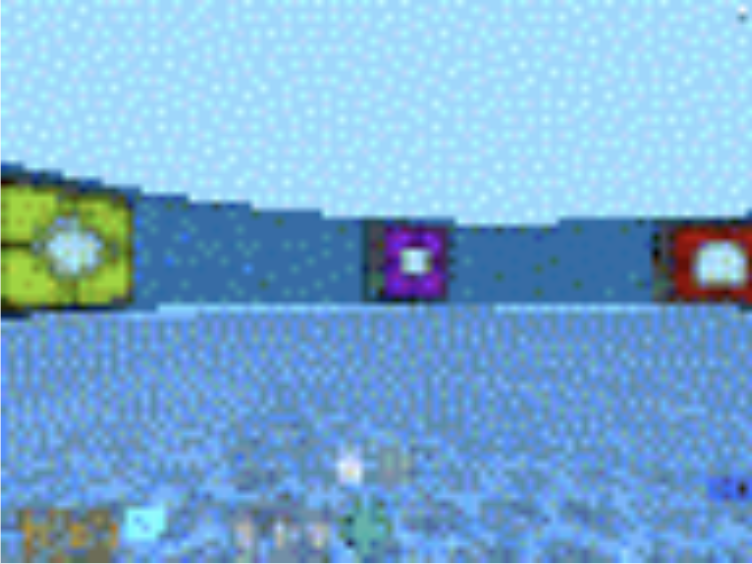
\includegraphics[width=0.27\textwidth]{assets/images/watermaze_env.png}
  \caption{\small Agent view from the DMLab Watermaze environment. The task is to find a hidden platform that elevates once found.
  }
 \vspace{-3mm}
\end{wrapfigure}
To investigate the in-context RL capabilities of \name and the baselines (see next section), we focus on environments that cannot be solved through zero-shot generalization after pre-training. Specifically, we require that each environment supports many tasks, that the tasks cannot be inferred easily from the observation, and that episodes are short enough to feasibly train across-episodic causal transformers - for more details regarding environments see Appendix~\ref{app:envs}. We list the evaluation environments below: 
 \\[2mm]
 {\bf Adversarial Bandit:} a multi-armed bandit with $10$ arms and $100$ trials similar to the environment considered in RL$^2$~\citep{duan2016rl2}. However, during evaluation the reward is out of distribution. Reward is more likely distributed under odd arms $95\%$ of the time during training. At evaluation, the opposite happens - reward appears more often under even arms $95\%$ of the time. 


{\bf Dark Room:} a 2D discrete POMDP where an agent spawns in a room and must find a goal location. The agent only knows its own $(x, y)$ coordinates but does not know the goal location and must infer it from the reward. The room size is $9\times9$, the possible actions are one step left, right, up, down, and no-op, the episode length is $20$, and the agent resets at the center of the map. We test two environment variants -- Dark Room where the agent receives $r=1$ every time the goal is reached and Dark Room Hard, a hard exploration variant with a $17\times17$ size and sparse reward ($r=1$ exactly once for reaching the goal). When not $r=1$, then $r=0$.


{\bf Dark Key-to-Door:} similar to Dark Room but this environment requires an agent to first find an invisible key upon which it receives a reward of $r=1$ once and then open an invisible door upon which it receives a reward of $r=1$ once again. Otherwise, the reward is $r=0$. The room size is $9\times 9$ making the task space combinatorial with $81^2=6561$ possible tasks. This environment is similar to the one considered in~\citet{chen2021dt} except the key and door are invisible and the reward is semi-sparse ($r=1$ for both key and the door). The agent is randomly reset. The episode length is $50$ steps.
\looseness=-1


{\bf DMLab Watermaze:} a partially observable 3D visual DMLab environment based on the classic Morris Watermaze~\citep{morris1981watermaze}. The task is to navigate the water maze to find a randomly spawned trap-door. The maze walls have color patterns that can be used to remember the goal location. Observations are pixel images of size $72\times96\times3$. There are 8 possible actions in total, including going forward, backward, left, or right, rotating left or right, and rotating left or right while going forward. The episode length is 50, and the agent resets at the center of the map. Similar to Dark Room, the agent cannot see the location of the goal from the observations and must infer it through the reward of $r=1$ if reached and $r=0$ otherwise; however, the goal space is continuous and therefore there are an infinite number of goals.


\subsection{Baselines}
\label{subsec:experimental-setup:baselines}

    The main aim of this work is to investigate to what extent \name reinforcement learns in-context relative to prior related work. \name is mostly closely related to Policy Distillation, where a policy is learned with a sequential model from offline interaction data. In-context online meta-RL is also related though not directly comparable to \namenospace, since \name is an in-context \emph{offline} meta-RL method. Still, we consider both types of baselines to better contextualize our work. For a more detailed discussion of these baseline choices we refer the reader to Appendix~\ref{app:baselines}. Our baselines include:


{\it Expert Distillation (ED):}  this baseline is exactly the same as \name but the source data consists of expert trajectories only, rather than learning histories. ED is most similar to Gato~\citep{reed2022gato} except ED models state-action-reward sequences like \namenospace, while Gato models state-action sequences. 

{\it Source Algorithm:}  we compare \name to the  gradient-based source RL algorithm that generates the training data for distillation. We include running the source algorithm from scratch as a baseline to compare the data-efficiency of in-context RL to the in-weights source algorithm.

{\it $\text{RL}^2$~\citep{duan2016rl2}:}  an online meta-RL algorithm where exploration and fast in-context adaptation are learned jointly by maximizing a multi-episodic value function. $\text{RL}^2$ is not directly comparable to \name for similar reasons to why online and offline RL algorithms are not directly comparable -- $\text{RL}^2$ gets to interact with the environment during training while \name does not. We use $\text{RL}^2$ asymptotic performance as an approximate upper bound for \namenospace. 


\begin{figure}[t]
\centering
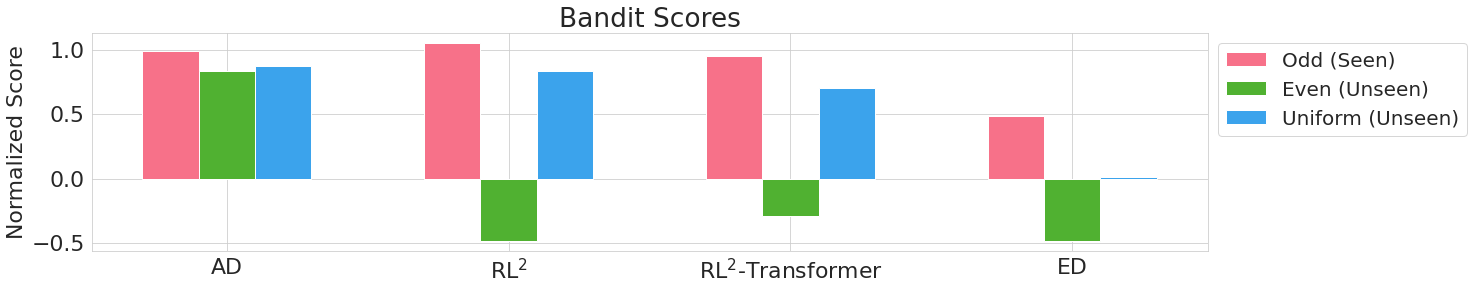
\includegraphics[width=1.0\textwidth]{assets/images/bandit.png}
\caption{\small {\it Adversarial Bandit (Section~\ref{sec:exps}):} \namenospace, $\text{RL}^2$, and ED evaluated on a $10$-arm bandit with $100$ trials. The source data for \name comes from learning histories from UCB~\citep{lai86ucb}. During training, the reward is distributed under odd arms $95\%$ of the time and under even arms $95\%$ of the time during evaluation. Both \name and $\text{RL}^2$ can in-context learn in-distribution tasks, but \name generalizes better out of distribution. Running $\text{RL}^2$ with a transformer generally doesn't offer an advantage over the original LSTM variant. ED performs poorly both in and out of distribution relative to \name and $\text{RL}^2$. Scores are normalized relative to UCB.}
\label{fig:bandit}
\end{figure}


\subsection{Evaluation}

After pre-training, the \name transformer $\algo_\theta$ can reinforcement learn in-context. Evaluation is exactly the same as with an in-weights RL algorithm except the learning happens entirely in-context without updating the transformer network parameters. Given an MDP (or POMDP), the transformer interacts with the environment and populates its own context (\ie \ without demonstrations), where the context is a queue containing the last $c$ transitions. The transformer's performance is then evaluated in terms of its ability to maximize return. For all evaluation runs, we average results across 5 training seeds with 20 evaluation seeds each for a total of 100 seeds. A task $\mathcal M$ is sampled uniformly from the test task distribution and fixed for each evaluation seed. The aggregate statistics reported reflect multi-task performance. We evaluate for 1000 and 160 episodes for the Dark and Watermaze environments respectively and plot performance as a function of total environment steps at test-time. 

